\documentclass[14pt, draft, oneside]{extreport}
\usepackage[utf8]{inputenc}
\usepackage[russianb]{babel}
\usepackage{vmargin}
\setpapersize{A4}
\setmarginsrb{2cm}{1.5cm}{1cm}{1.5cm}{0pt}{0mm}{0pt}{13mm}
\usepackage{indentfirst}
\usepackage{graphicx}
\fussy
\begin{document}
\tableofcontents

\chapter{Введение}
\section{Назначение}

Операционная система, написанная в ходе работы над курсовой работой,
является примером операционной системы реального времени с полным 
переключением контекста, полностью удовлетворяющая 
функциональной спецификации.
Для реализации был выбран вытесняющий алгоритм планирования задач.

\section{Задание}

Необходимо реализовать модель операционной системы реального 
времени, обладающей следующими свойствами:

\begin{itemize}
    \item \textbf{Тип планировщика}: POSIX
    \item \textbf{Алгоритм планирования}: preemtive, RMA
    \item \textbf{Управление ресурсами}: HLP
    \item \textbf{Управление событиями}: нет
    \item \textbf{Обработка прерываний}: есть, допустимо объявление
        локальных переменных
    \item \textbf{Макс. кол-во задач}: 32
    \item \textbf{Макс. кол-во приоритетов}: 16
    \item \textbf{Макс. кол-во ресурсов}: 16
\end{itemize}

\section {Средства реализации}

Проект был реализован на языке программирования C с полным
соответсвием стандарту ISO/ANSI C с использованием компилятора 
GCC версии 15.1.1.

\chapter{Описание структуры проекта}
\section{Управление ОС}
\begin{itemize}
    \item \textbf{StartOS}: Запуск ОС, инициализация основных
        элементов системы, активация начальной задачи
    \item \textbf{ShutdownOS}: Завершение работы ОС
\end{itemize}

\section{Управление задачами}

\begin{itemize}
    \item \textbf{ActivateTask}: Инициализация задачи в системе
    \item \textbf{TerminateTask}: Завершение задачи
    \item \textbf{Schedule}: Постановка задачи в очередь
    \item \textbf{Dispatch}: Диспетчеризация задач, постановка в 
        очередь на выполнение
\end{itemize}

\section{Управление ресурсами}

\begin{itemize}
    \item \textbf{InitRes}: Инициализация ресурса в системе
    \item \textbf{HLPGetRes}: Захват ресурса выполняющейся задачей
    \item \textbf{HLPReleaseRes}: Освобождение ресурса
\end{itemize}

\section{Обработка прерываний}

\begin{itemize}
    %TODO: Точно ли клавиатуры??? Может клавиши или кнопки или прям
    %      <Ctrl-C>??
    \item \textbf{ISRSetHandler}: Установка прерывания клавиатуры
    \item \textbf{ISRClearHandler}: Сброс прерывания клавиатуры
\end{itemize}

\chapter {Вытесняющий алгоритм планирования}

\begin{figure}[h]
    \centering
    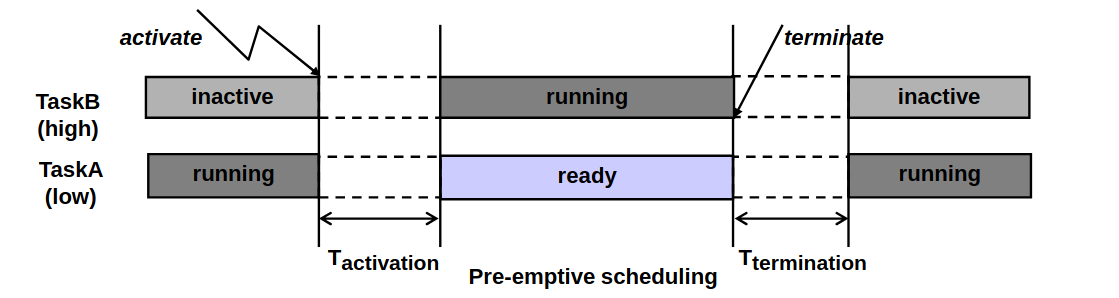
\includegraphics[width=0.9\textwidth]{{pictures/algorithm}.png}
    \caption{Принцип работы вытесняющего алгоритма планирования}
\end{figure}

\chapter {Тестирование}
\section{Тест-кейс №1}

\use{test/test1.tex}

\section{Тест-кейс №2}

\use{test/test2.tex}

\section{Тест-кейс №3}

\use{test/test3.tex}

\section{Тест-кейс №4}

\use{test/test4.tex}


\end{document}
